\documentclass[11pt]{article}
\usepackage[margin=1in]{geometry}
\usepackage{amsmath,amssymb,graphicx,booktabs,listings,xcolor}
\setlength{\parindent}{0pt}\setlength{\parskip}{5pt}

\lstset{
  language=Matlab,
  basicstyle=\ttfamily\footnotesize,
  commentstyle=\color{gray},
  keywordstyle=\color{blue!60!black},
  frame=single,
  framerule=0.3pt,
  breaklines=true,
  columns=fullflexible,
  aboveskip=6pt, belowskip=6pt
}

\newcommand{\bmat}[1]{\begin{bmatrix}#1\end{bmatrix}}

\title{RBE 502 -- Homework 2}
\author{Shreehan}
\date{September 2026}

\begin{document}
\maketitle

All code is in the \texttt{matlab/} folder of the repo (one file per problem, \texttt{hw2\_p1.m} to \texttt{hw2\_p6.m}). The snippets below are only the key parts.

\section*{Problem 1}

For each system I linearized at the origin, $A=\partial f/\partial x\big|_{x=0}$, and looked at the eigenvalues. If every $\mathrm{Re}(\lambda)<0$ the origin is asymptotically stable. The $x_1x_2$ and $x_2^3$ terms drop out of $A$ since their slope is zero at $0$, and in systems 2 and 3 the factors $(1-x_1^2-x_2^2)$ and $(1-x_1^2)$ just evaluate to $1$ after the product rule.

\begin{center}
\begin{tabular}{clll}
\toprule
 & $A$ & char.\ polynomial & eigenvalues\\
\midrule
1 & $\bmat{-1&0\\0&-1}$ & $(\lambda+1)^2$ & $-1,\,-1$\\[6pt]
2 & $\bmat{-1&-1\\1&-1}$ & $\lambda^2+2\lambda+2$ & $-1\pm j$\\[6pt]
3 & $\bmat{0&1\\-1&-1}$ & $\lambda^2+\lambda+1$ & $-\tfrac12\pm j\tfrac{\sqrt3}{2}$\\[6pt]
4 & $\bmat{-1&-1\\2&0}$ & $\lambda^2+\lambda+2$ & $-\tfrac12\pm j\tfrac{\sqrt7}{2}$\\
\bottomrule
\end{tabular}
\end{center}

All real parts are negative, so the origin is asymptotically stable for all four systems.

\begin{lstlisting}
J = jacobian(f, x);
J_at_origin = subs(J, x, [0; 0]);
A{i} = double(J_at_origin);
eigenvalues = eig(A{i});
\end{lstlisting}

\section*{Problem 2}

Set $f(x)=0$ to get the equilibria, then linearize at each one and check the eigenvalues of the Jacobian.

\textbf{System 1.} $\dot x_2=0$ gives $x_2=3x_1$, so $x_1(4-x_1^2)=0$ and $x_1\in\{0,\pm2\}$. With $J=\bmat{1-3x_1^2&1\\3&-1}$:
\begin{itemize}
\item $(0,0)$: $\lambda=\pm2$, saddle.
\item $(\pm2,\pm6)$: $\lambda^2+12\lambda+8=0$, $\lambda=-6\pm2\sqrt7$, stable node.
\end{itemize}

\textbf{System 2.} From $x_2(x_1-x_2)=0$: either $x_2=0$ (then $x_1=2$ or $-4$) or $x_2=x_1$ (then $x_1=2$ or $4$). $J=\bmat{2x_1-2x_2+2&-2x_1+4\\x_2&x_1-2x_2}$.
\begin{center}
\begin{tabular}{lll}
\toprule
equilibrium & eigenvalues & type\\
\midrule
$(2,0)$ & $6,\,2$ & unstable node\\
$(-4,0)$ & $-6,\,-4$ & stable node\\
$(2,2)$ & $2,\,-2$ & saddle\\
$(4,4)$ & $-1\pm j\sqrt7$ & stable focus\\
\bottomrule
\end{tabular}
\end{center}

\textbf{System 3.} $x_2(3-x_1-2x_2)=0$ and $x_1(2-x_1-x_2)=0$ give $(0,0)$, $(2,0)$, $(0,\tfrac32)$ and $(1,1)$. $J=\bmat{-x_2&3-x_1-4x_2\\2-2x_1-x_2&-x_1}$.
\begin{center}
\begin{tabular}{lll}
\toprule
equilibrium & eigenvalues & type\\
\midrule
$(0,0)$ & $\pm\sqrt6$ & saddle\\
$(2,0)$ & $-1\pm j$ & stable focus\\
$(0,\tfrac32)$ & $-\tfrac34\pm j\tfrac{\sqrt{15}}{4}$ & stable focus\\
$(1,1)$ & $-1\pm\sqrt2$ & saddle\\
\bottomrule
\end{tabular}
\end{center}

\textbf{System 4.} Let $a(x)=\tfrac12\tan(\pi x/2)$. The equilibrium conditions are $x_2=a(x_1)$ and $x_1=a(x_2)$. Subtracting them gives $x_2+a(x_2)=x_1+a(x_1)$, and since $x+a(x)$ is strictly increasing on $(-1,1)$ this forces $x_1=x_2=x$ with $\tan(\pi x/2)=2x$. The roots are $x=0,\pm\tfrac12$ (it is convex for $x>0$ with a negative slope at $0$, so there is only one positive root). The Jacobian is
\[
J=\bmat{-c&1\\1&-c},\qquad c=\tfrac{\pi}{4}\sec^2\!\big(\tfrac{\pi x}{2}\big),
\]
with eigenvalues $-c\pm1$.
\begin{itemize}
\item $(0,0)$: $c=\pi/4<1$, so $\lambda=-\tfrac\pi4\pm1=0.215,\,-1.785$, saddle.
\item $(\pm\tfrac12,\pm\tfrac12)$: $c=\pi/2$, so $\lambda=-0.571,\,-2.571$, stable node.
\end{itemize}
I only looked at $|x_i|<1$, the principal branch of $\tan$. The field has more equilibria on the other branches (for example $x_1=x_2\approx2.89$), and they are all stable nodes since $c>1$ there.

\begin{lstlisting}
sol = solve(f == 0, [x1 x2]);      % systems 1-3
xe  = double([sol.x1, sol.x2]);    % one equilibrium per row
A   = double(subs(J, x, xe(k,:).'));

g = @(t) t - 0.5*tan(pi*t/2);      % system 4, with x1 = x2 = t
r = fzero(g, [xs(k) xs(k+1)]);     % bracket from a sign change
\end{lstlisting}

\section*{Problem 3}

Same approach as Problem 1, just with three states.

\begin{enumerate}
\item $A=\mathrm{diag}(-1,-1,1)$. The $-x_1^2$ in $\dot x_3$ has zero slope at $0$. One eigenvalue is $+1$, so the origin is \textbf{unstable}.
\item $A=\bmat{-1&0&0\\-1&-1&-1\\0&1&0}$. It is block lower triangular, so $\det(\lambda I-A)=(\lambda+1)(\lambda^2+\lambda+1)$ and $\lambda=-1,\,-\tfrac12\pm j\tfrac{\sqrt3}{2}$. \textbf{Asymptotically stable.}
\item $A=\mathrm{diag}(-2,-1,-1)$. \textbf{Asymptotically stable.}
\end{enumerate}

\begin{lstlisting}
A  = double(subs(jacobian(f, x), x, [0; 0; 0]));
re = real(eig(A));
if all(re < -tol),     disp('asymptotically stable');
elseif any(re > tol),  disp('unstable');
else,                  disp('inconclusive'); end
\end{lstlisting}

\section*{Problem 4}

For $u=-Kx$ I wrote $A_{cl}=A-BK$ and matched $\det(sI-A_{cl})$ against the desired polynomial.

\subsection*{(a) Linear system}

$\det(\lambda I-A)=(\lambda-1)^2-9$, so $\lambda=4,-2$ and the open loop is unstable. The controllability matrix is $[B\;AB]=\bmat{1&1\\0&3}$ with determinant $3$, so the system is controllable.

With $A_{cl}=\bmat{1-k_1&3-k_2\\3&1}$,
\[
\det(sI-A_{cl})=s^2+(k_1-2)s-k_1+3k_2-8 .
\]
The desired poles $-1\pm2j$ give $s^2+2s+5$. So $k_1-2=2$ gives $k_1=4$, and $-4+3k_2-8=5$ gives $k_2=17/3$.
\[
K=\bmat{4&\tfrac{17}{3}}
\]

\subsection*{(b) DC motor}

With the given numbers $A=\bmat{-4&0.2\\10&-2}$ and $B=\bmat{2\\0}$ (I used $A$ as printed in the assignment, with $+K/L$ in the top right). Then $\lambda^2+6\lambda+6=0$, so $\lambda=-3\pm\sqrt3$ and the open loop is asymptotically stable. $[B\;AB]=\bmat{2&-8\\0&20}$ has determinant $40$, so it is controllable.

$A_{cl}=\bmat{-4-2k_1&0.2-2k_2\\10&-2}$ gives
\[
\det(sI-A_{cl})=s^2+(6+2k_1)s+6+4k_1+20k_2 .
\]
The desired poles $-5\pm5j$ give $s^2+10s+50$. So $k_1=2$, and $6+8+20k_2=50$ gives $k_2=9/5$.
\[
K=\bmat{2&1.8}
\]
If the motor is meant to have $-K/L$ in that entry instead, the same steps give $k_2=1.6$.

\begin{lstlisting}
Acl      = A - B*[k1 k2];
char_cl  = expand(det(s*eye(2) - Acl));
char_des = pd(1)*s^2 + pd(2)*s + pd(3);
sol      = solve(coeffs(char_cl - char_des, s), [k1 k2]);
K        = place(A, B, p);          % check
\end{lstlisting}

\texttt{place} returns the same gains, and the closed-loop eigenvalues come out at the requested poles.

\section*{Problem 5}

State is $z=[x,\theta,\dot x,\dot\theta]^T$, and I use $D=I(M+m)+Mml^2=(m+M)(I+ml^2)-m^2l^2$.

\subsection*{1. Small-angle linearization}

With $\cos\theta\approx1$, $\sin\theta\approx\theta$ and $\dot\theta^2\sin\theta\approx0$ the equations become
\[
(m+M)\ddot x+ml\ddot\theta=F,\qquad (I+ml^2)\ddot\theta+ml\ddot x=mgl\,\theta .
\]
Solving the two for the accelerations:
\[
\ddot x=\frac{(I+ml^2)F-m^2gl^2\theta}{D},\qquad
\ddot\theta=\frac{mgl(M+m)\theta-mlF}{D}.
\]
\[
A=\bmat{0&0&1&0\\0&0&0&1\\0&-\frac{m^2gl^2}{D}&0&0\\0&\frac{mgl(M+m)}{D}&0&0},\qquad
B=\bmat{0\\0\\\frac{I+ml^2}{D}\\-\frac{ml}{D}}
\]

\subsection*{2. Nonlinear form and Taylor expansion}

Solving the exact equations for $\ddot x$ and $\ddot\theta$, with $\Delta(\theta)=D+m^2l^2\sin^2\theta$:
\begin{align*}
\ddot x&=\frac{(I+ml^2)F+ml(I+ml^2)\dot\theta^2\sin\theta-m^2gl^2\sin\theta\cos\theta}{\Delta(\theta)},\\
\ddot\theta&=\frac{ml\,[\,-F\cos\theta+(M+m)g\sin\theta-ml\dot\theta^2\sin\theta\cos\theta\,]}{\Delta(\theta)},
\end{align*}
and $\dot z=[\dot x,\dot\theta,\ddot x,\ddot\theta]^T$. At $z=0$, $F=0$ both numerators are zero, so the derivative of $\Delta$ does not matter, and $\partial\Delta/\partial\theta=0$ there anyway. The terms with $\dot\theta^2$ vanish as well. What is left is
\[
\frac{\partial\ddot x}{\partial\theta}=-\frac{m^2gl^2}{D},\quad
\frac{\partial\ddot\theta}{\partial\theta}=\frac{mgl(M+m)}{D},\quad
\frac{\partial\ddot x}{\partial F}=\frac{I+ml^2}{D},\quad
\frac{\partial\ddot\theta}{\partial F}=-\frac{ml}{D},
\]
which is the same $A$ and $B$ as in part 1. The code also checks this symbolically.

\subsection*{3. State feedback}

With $m=0.16$, $M=0.48$, $l=0.5$, $g=9.8$, $I=\tfrac1{12}ml^2$:
\[
A=\bmat{0&0&1&0\\0&0&0&1\\0&-2.94&0&0\\0&23.52&0&0},\qquad
B=\bmat{0\\0\\2.03125\\-3.75}.
\]
The open-loop eigenvalues are $0,0,\pm4.85$, so it is unstable. The controllability matrix has full rank (4), so poles can be placed anywhere. I picked $\{-2,-3,-4,-5\}$, i.e.\ $s^4+14s^3+71s^2+154s+120$, and got
\[
K=\bmat{-3.265&-26.974&-4.190&-6.003},\qquad F=-Kz .
\]
I also simulated the full nonlinear model with this controller from $\theta_0=0.1$ and $0.3$\,rad, and both go back to zero (Fig.~\ref{fig:p5}).

\textbf{Symbolic gain (bonus).} Write $a=-\tfrac{m^2gl^2}{D}$, $b=\tfrac{mgl(M+m)}{D}$, $c=\tfrac{I+ml^2}{D}$, $d=-\tfrac{ml}{D}$. Expanding $\det(sI-A+BK)$ gives
\[
s^4+(ck_3+dk_4)s^3+(-b+ck_1+dk_2)s^2+(ad-bc)k_3\,s+(ad-bc)k_1 ,
\]
and $ad-bc=-glm/D$. Matching to $s^4+p_3s^3+p_2s^2+p_1s+p_0$:
\[
k_1=-\frac{D\,p_0}{glm},\quad
k_3=-\frac{D\,p_1}{glm},\quad
k_2=\frac{p_2+b-c\,k_1}{d},\quad
k_4=\frac{p_3-c\,k_3}{d}.
\]
Plugging in the numbers gives the same $K$ as \texttt{place}.

\begin{lstlisting}
A0 = simplify(subs(jacobian(f, z), vars, [0 0 0 0 0]));   % Taylor
B0 = simplify(subs(diff(f, F),     vars, [0 0 0 0 0]));
K  = place(An, Bn, [-2 -3 -4 -5]);
cp = expand(det(s*eye(4) - (A_s - B_s*[k1 k2 k3 k4])));
Ks = solve(coeffs(cp - cdes, s), [k1 k2 k3 k4]);          % symbolic gains
\end{lstlisting}

\begin{figure}[h]
\centering
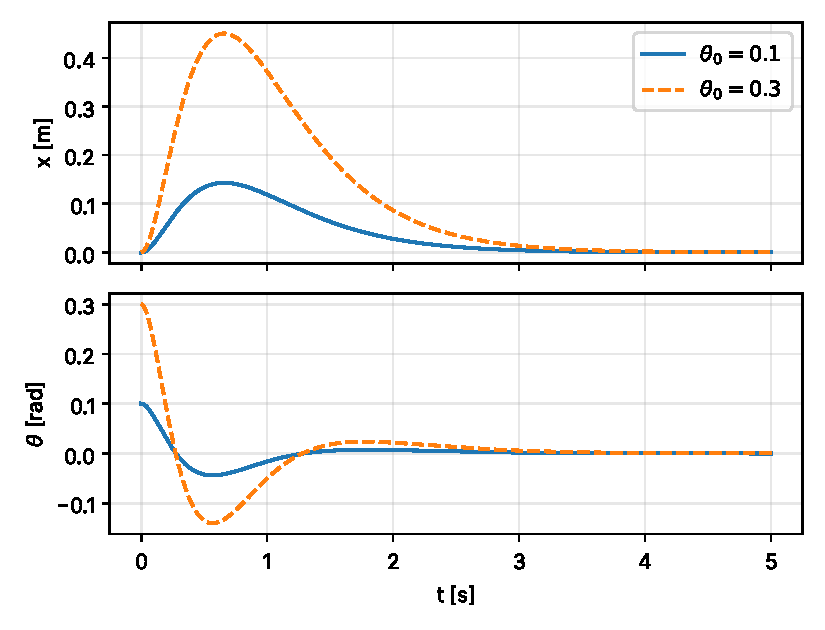
\includegraphics[width=0.6\linewidth]{figures/p5.pdf}
\caption{Nonlinear cart-pendulum with $F=-Kz$.}
\label{fig:p5}
\end{figure}

\subsection*{4. (Bonus) Equations of motion}

Take the pendulum center of mass at $(x+l\sin\theta,\;l\cos\theta)$. Then
\[
T=\tfrac12(M+m)\dot x^2+ml\dot x\dot\theta\cos\theta+\tfrac12(I+ml^2)\dot\theta^2,\qquad V=mgl\cos\theta,
\]
and the generalized forces are $Q_x=F$, $Q_\theta=0$. Lagrange's equation for $x$ gives $(M+m)\ddot x+ml\ddot\theta\cos\theta-ml\dot\theta^2\sin\theta=F$. For $\theta$ the $ml\dot x\dot\theta\sin\theta$ terms cancel and you get $(I+ml^2)\ddot\theta+ml\ddot x\cos\theta-mgl\sin\theta=0$. Both match the given equations.

\subsection*{5. (Bonus) Linearization at $\theta=\pi$}

Let $\varphi=\theta-\pi$, so $\sin\theta\approx-\varphi$ and $\cos\theta\approx-1$:
\[
(m+M)\ddot x-ml\ddot\varphi=F,\qquad (I+ml^2)\ddot\varphi-ml\ddot x+mgl\,\varphi=0 .
\]
Solving gives
\[
\ddot x=\frac{(I+ml^2)F-m^2gl^2\varphi}{D},\qquad
\ddot\varphi=\frac{mlF-mgl(M+m)\varphi}{D}.
\]
So $A$ is the same as before except the $(4,2)$ entry flips sign, and the last entry of $B$ is $+ml/D$. The Taylor expansion gives the same thing. Now the lower block is oscillatory, $\lambda=\pm j4.85$, which makes sense for a pendulum hanging down.

\section*{Problem 6}

The model is $\dot x=\nu\cos\theta$, $\dot y=\nu\sin\theta$, $\dot\theta=\omega$, $\dot\nu=u_1$, $\dot\omega=u_2$, with $V=\mathbf{x}^T\mathbf{x}$ where $\mathbf{x}=[x,y,\theta,\nu,\omega]^T$.

\subsection*{1. Derivative of $V$}

\[
\dot V=2\mathbf{x}^T\dot{\mathbf{x}}
=2\big[x\nu\cos\theta+y\nu\sin\theta+\theta\omega+\nu u_1+\omega u_2\big].
\]

\subsection*{2. The given control law}

Putting in $u_1=-k_1\nu-x\cos\theta-y\sin\theta$ and $u_2=-k_2\omega-\theta$:
\[
\nu u_1=-k_1\nu^2-x\nu\cos\theta-y\nu\sin\theta,\qquad \omega u_2=-k_2\omega^2-\theta\omega ,
\]
so the cross terms cancel and
\[
\dot V=-2k_1\nu^2-2k_2\omega^2\le0 .
\]
$V$ is positive definite and radially unbounded, so the origin is stable and trajectories stay bounded. But $\dot V$ is only negative semidefinite (it is zero whenever $\nu=\omega=0$), so this does not give asymptotic stability. I used LaSalle.

On $\{\dot V=0\}=\{\nu=\omega=0\}$, staying there requires $\dot\omega=u_2=-\theta=0$, so $\theta\equiv0$, and $\dot\nu=u_1=-x\cos\theta-y\sin\theta=-x=0$, so $x\equiv0$. Nothing forces $y$ to zero, so the largest invariant set is
\[
\mathcal M=\{(0,\,y,\,0,\,0,\,0):\ y\in\mathbb R\}.
\]
Every point in $\mathcal M$ is an equilibrium of the closed loop, so trajectories converge to \emph{some} point on that line but not necessarily the origin.

\textbf{Conclusion: this controller does not asymptotically stabilize the origin.}

\emph{Quantitative.} The equilibrium set is a whole line, so the origin is not isolated and cannot be asymptotically stable. Linearizing the closed loop at $0$ gives $\ddot x=-k_1\dot x-x$, $\ddot\theta=-k_2\dot\theta-\theta$ and $\dot y\approx0$, so the eigenvalues are the roots of $s^2+k_1s+1$, $s^2+k_2s+1$ and an extra $s=0$ from $y$. In simulation with $k_1=k_2=1$ (Fig.~\ref{fig:p6}) the states $x,\theta,\nu,\omega$ all go to zero but $y$ ends at $0.664$, $-0.949$ and $1.435$ for the three initial conditions I tried, and $V$ decreases but does not reach zero.

\emph{Qualitative.} The robot cannot move sideways, so $y$ only changes when $\nu\sin\theta\neq0$. The controller drives $\theta$ and $\nu$ to zero, which freezes $y$ wherever it happens to be. This is the usual nonholonomic problem: no smooth static feedback can asymptotically stabilize this kind of system (Brockett), so you need something time-varying or discontinuous.

\begin{lstlisting}
Vdot = simplify(expand(2*q.'*f_cl));      % -2*k1*nu^2 - 2*k2*om^2
[t, S] = ode45(dyn, [0 200], inits{i}, opts);
\end{lstlisting}

\begin{figure}[h]
\centering
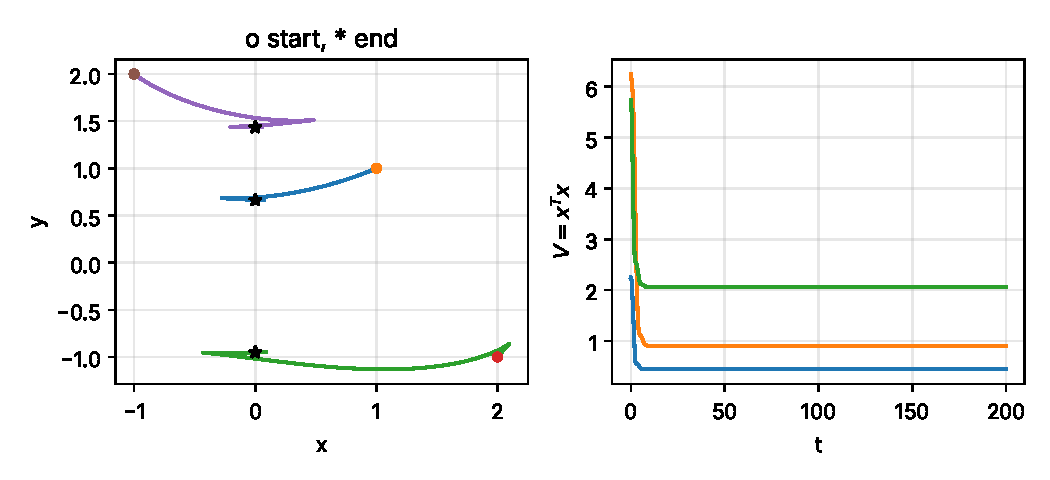
\includegraphics[width=0.85\linewidth]{figures/p6.pdf}
\caption{Closed-loop trajectories end on the line $x=\theta=0$ at $y\neq0$ (left); $V$ does not go to zero (right).}
\label{fig:p6}
\end{figure}


\end{document}
